
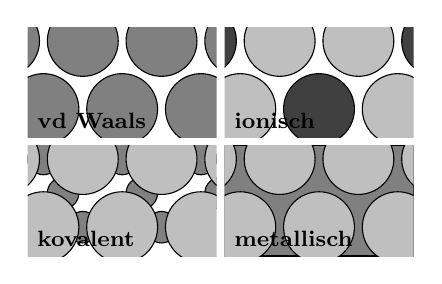
\begin{tikzpicture}

%\useasboundingbox (-1.3,-1.2) rectangle (11.2,4.7);
%	\draw (-1.5,-2.5) rectangle (3.5,7.5);


\begin{scope}[yshift=0mm]
  
 \clip (3mm,5mm) rectangle ++ (24mm, 14mm);  
   
 \foreach \u in {1,2,...,7}{%  
     \foreach \v in {1,2,...,4}{%  
            \draw[fill=gray] ({\u + \v * cos(120)}, {\v * sin(120) } )  circle (4.5mm) node (o\u\v) {};
         }
  }
  
     \node[anchor=south west] at (3mm,5mm) {\footnotesize \bf vd Waals};

\end{scope}

\begin{scope}[xshift=25mm]
  
 \clip (3mm,5mm) rectangle ++ (24mm, 14mm);  
   
 
    \draw[fill=gray!50!white] ({1 + 1 * cos(120)}, {1* sin(120) } )  circle (4.5mm) ;
    \draw[fill=gray!50!black] ({2 + 1 * cos(120)}, {1* sin(120) } )  circle (4.5mm) ;
        \draw[fill=gray!50!white] ({3 + 1 * cos(120)}, {1* sin(120) } )  circle (4.5mm) ;

    \draw[fill=gray!50!black] ({1 + 2 * cos(120)}, {2* sin(120) } )  circle (4.5mm) ;
    \draw[fill=gray!50!white] ({2 + 2 * cos(120)}, {2* sin(120) } )  circle (4.5mm) ;
    \draw[fill=gray!50!white] ({3 + 2 * cos(120)}, {2* sin(120) } )  circle (4.5mm) ;
            \draw[fill=gray!50!black] ({4 + 2 * cos(120)}, {2* sin(120) } )  circle (4.5mm) ;
 
    \node[anchor=south west] at (3mm,5mm) {\footnotesize \bf ionisch};

  
\end{scope}

\begin{scope}[yshift=-15mm]
  
 \clip (3mm,5mm) rectangle ++ (24mm, 14mm);  
   
 \foreach \u in {1,2,...,7}{%  
     \foreach \v in {1,2,...,4}{%  
            \draw[fill=gray] ({0.5 + \u + \v * cos(120)}, {\v * sin(120) } )  circle (2mm) ;
            \draw[fill=gray] ({0.5 + \u + (0.5 + \v ) * cos(120)}, {(0.5 + \v ) * sin(120) } )  circle (2mm) ;
         }
  }   
   
 \foreach \u in {1,2,...,7}{%  
     \foreach \v in {1,2,...,4}{%  
            \draw[fill=gray!50!white] ({\u + \v * cos(120)}, {\v * sin(120) } )  circle (4.5mm) node (o\u\v) {};
         }
  }
  
     \node[anchor=south west] at (3mm,5mm) {\footnotesize \bf kovalent};

\end{scope}


\begin{scope}[yshift=-15mm,xshift=25mm]
  
 \clip (3mm,5mm) rectangle ++ (24mm, 14mm);  
   
   
  \draw[fill=gray] (3mm,5mm) rectangle ++ (24mm, 14mm);  
 
   
 \foreach \u in {1,2,...,7}{%  
     \foreach \v in {1,2,...,4}{%  
            \draw[fill=gray!50!white] ({\u + \v * cos(120)}, {\v * sin(120) } )  circle (4.5mm) node (o\u\v) {};
         }
  }
   \node[anchor=south west] at (3mm,5mm) {\footnotesize \bf metallisch};
 
\end{scope}

  \end{tikzpicture}




